\section{Архитектура безопасности Android}

Операционная система Android изначально разрабатывалась с учётом принципов
безопасности и гибкой архитектуры. С каждым обновлением система включает всё
более продвинутые механизмы защиты пользовательских данных. Начиналось всё с
элементарных вещей. Таких как PIN экрана, запуск приложения в изолированной
среде, указания определенных полномочий в конфигурационных файлах приложения.
Теперь архитектура безопасности Android представляет собой многоуровневую
структуру, включающую защиту на аппаратном уровне, уровне ядра операционной
системы, уровне приложений и уровне пользовательских данных. Все эти уровни
взаимодействуют друг с другом, создавая комплексную систему обеспечения
безопасности.

Android использует модель \textit{Defense in Depth} --- принцип многоуровневой
защиты, при котором один уровень безопасности дополняет и страхует другой. Эта
модель включает следующие уровни:

\begin{itemize}
    \item \textbf{Аппаратный уровень безопасности.} Реализуется функциями
    процессора и сопроцессоров (например, ARM TrustZone, Secure Element, Titan
    M). Доверенная среда выполнения (Trusted Execution Environment, TEE)
    позволяет изолированно выполнять критические операции, включая работу с
    криптографическими ключами.

    \item \textbf{Ядро операционной системы.} Android использует ядро Linux,
    обеспечивающее изоляцию процессов, управление доступом и защиту памяти. Все
    приложения работают в песочницах, каждый процесс имеет свой UID.
    Security-Enhanced Linux (SELinux) реализует обязательную модель управления
    доступом, ограничивая действия процессов и контролируя взаимодействие
    компонентов.

    \item \textbf{Android Keystore.} Система безопасного хранения и управления
    криптографическими ключами. Может использовать аппаратную изоляцию и
    предоставляет API для безопасного выполнения операций.

    \item \textbf{Уровень приложений.} Каждое приложение изолировано, работает
    в своей виртуальной машине (Android Runtime), доступ к чувствительным
    данным регулируется системой разрешений. С Android 6.0 разрешения можно
    выдавать и отзывать вручную.
\end{itemize}

Рисунок \ref{fig:fig01} иллюстрирует компоненты безопасности и аспекты защиты
на различных уровнях программного стека Android. Каждый компонент предполагает,
что компоненты, расположенные ниже, надёжно защищены. За исключением небольшого
объёма кода операционной системы Android, выполняемого от имени
root-пользователя, весь остальной код, находящийся выше ядра Linux, ограничен
Песочницей приложений (Application Sandbox).

\begin{figure}
    \centering
    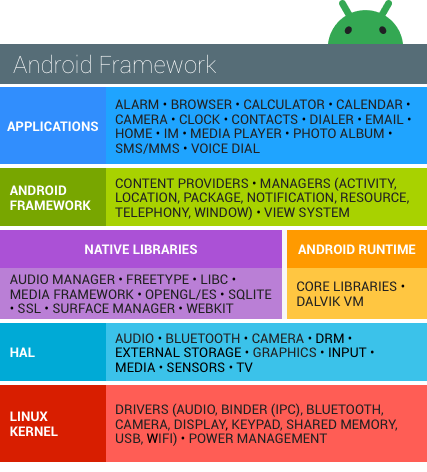
\includegraphics[scale=0.6]{inc/android-software-stack.png}
    \caption{ Программный стек Android }
    \label{fig:fig01}
\end{figure}

Таким образом, архитектура безопасности Android представляет собой целостную
систему, где каждый уровень выполняет свою роль, а шифрование служит основой
защиты пользовательских данных на всех этапах: от хранения до исполнения.
